\documentclass[aspectratio=169,12pt]{beamer}

\usetheme{Madrid}
\usecolortheme{default}
\useinnertheme{circles}

\definecolor{iiitblue}{RGB}{0,51,102}
\definecolor{migared}{RGB}{214,96,77}
\definecolor{miceblue}{RGB}{33,102,172}
\definecolor{migagreen}{RGB}{77,172,38}

\setbeamercolor{palette primary}{bg=iiitblue,fg=white}
\setbeamercolor{palette secondary}{bg=iiitblue!80,fg=white}
\setbeamercolor{palette tertiary}{bg=iiitblue!60,fg=white}
\setbeamercolor{palette quaternary}{bg=iiitblue,fg=white}
\setbeamercolor{frametitle}{bg=iiitblue,fg=white}
\setbeamercolor{title}{fg=iiitblue}
\setbeamercolor{structure}{fg=iiitblue}
\setbeamercolor{alerted text}{fg=migared}

\usepackage[utf8]{inputenc}
\usepackage[T1]{fontenc}
\usepackage{mathpazo}
\usepackage{booktabs}
\usepackage{multirow}
\usepackage{amssymb}
\usepackage{graphicx}

\setbeamertemplate{navigation symbols}{}
\setbeamertemplate{footline}[frame number]

\newcommand{\MIGA}{\textsc{MIGA}}
\newcommand{\MICE}{\textsc{MICE}}
\newcommand{\Fr}{$F_r$}

%---------------------------------------------------------------------
\title[MIGA: Distributional Imputation]{Missing Data Imputation via Genetic Algorithms:\\
A Distributional Analysis of MIGA}
\author{Madhav Umesh Kamble \\ {\small Roll: MDE2025008}}
\institute[IIIT Allahabad]{
  Department of Information Technology \\
  Indian Institute of Information Technology, Allahabad \\[4pt]
  {\small Supervisor: Dr.\ Gaurav Srivastava}
}
\date{May 2026}
%---------------------------------------------------------------------

\begin{document}

\begin{frame}
  \titlepage
\end{frame}

%---------------------------------------------------------------------
\begin{frame}{Outline}
  \tableofcontents
\end{frame}

%---------------------------------------------------------------------
\section{Motivation}
%---------------------------------------------------------------------

\begin{frame}{The Missing Data Problem}

\begin{columns}
\begin{column}{0.55\textwidth}
\textbf{Three strategies — each with a cost}
\begin{enumerate}
  \item Delete incomplete rows \\
        {\small → selection bias, lost power}
  \item Mean imputation \\
        {\small → distorts variance}
  \item \MICE{} (iterative regression) \\
        {\small → minimises RMSE, but \alert{suppresses variance}}
\end{enumerate}

\bigskip
\textbf{The gap} \\
\MICE{} is optimal for RMSE. \\
Not for distributional correctness.
\end{column}

\begin{column}{0.42\textwidth}
\begin{block}{Van Buuren (2018, \S2.6)}
\small ``Regression imputation achieves minimum RMSE by suppressing variance and produces biased statistical inference.''
\end{block}

\bigskip
\begin{block}{MIGA (Information Sciences, 2023)}
\small Imputes by matching the \emph{joint distribution}, not minimising pointwise error.\\[4pt]
\textbf{No public code.} \\
No comparison vs \MICE{} or KNN. \\
No MNAR evaluation.
\end{block}
\end{column}
\end{columns}

\end{frame}

%---------------------------------------------------------------------
\section{MIGA Algorithm}
%---------------------------------------------------------------------

\begin{frame}{MIGA: Impute by Matching the Distribution}

\begin{columns}
\begin{column}{0.48\textwidth}
\textbf{Two subsets of the data:}
\begin{itemize}
  \item $X_A$ = complete rows (reference)
  \item $X_C$ = rows with $\geq 1$ missing value
\end{itemize}

\bigskip
\textbf{Fitness function (minimise):}
\[
F_r = \underbrace{D_r(\tilde{x}_A, \tilde{x}_C)}_{\text{means}} +
      \underbrace{D_r(\tilde{S}, I)}_{\text{covariance}} +
      \underbrace{D_r(b_A, b_C)}_{\text{skewness}}
\]
$\tilde{S} = S_A^{-1/2} S_C S_A^{-1/2}$ \\[3pt]
$F_r = 0 \Leftrightarrow X_C \overset{d}{=} X_A$
\end{column}

\begin{column}{0.48\textwidth}
\textbf{Genetic algorithm:}
\begin{itemize}
  \item $l = 200$ candidate imputations
  \item $G$ generations, $Q = 3$--$5$ runs
  \item Operators: selection, crossover, \\
        mutation ($c_3$), diversity injection
\end{itemize}

\bigskip
\begin{alertblock}{Key difference from MICE}
MIGA never sees the true missing values.
It only checks: does the imputed distribution match the reference?
\end{alertblock}
\end{column}
\end{columns}

\end{frame}

%---------------------------------------------------------------------
\section{Contributions}
%---------------------------------------------------------------------

\begin{frame}{Ten Contributions}

\renewcommand{\arraystretch}{1.25}
\begin{tabular}{clp{7.2cm}}
\toprule
\textbf{C} & \textbf{Type} & \textbf{Description} \\
\midrule
C1 & Reimplementation & First public MIGA code; 5 UCI datasets; fully reproducible \\
\textbf{C2} & \textbf{Theory} & \textbf{Formal proof: $F_r$--RMSE structural orthogonality} \\
\textbf{C3} & \textbf{Empirical} & \textbf{First MNAR evaluation of MIGA (4 mechanisms, 5 datasets)} \\
\textbf{C4} & \textbf{Empirical} & \textbf{$F_r$ vs RMSE comparison + Wilcoxon significance (10 seeds)} \\
\textbf{C5} & \textbf{Empirical} & \textbf{Synthetic $p \times \rho$ grid — dimension-correlation interaction} \\
C6 & Engineering & IPW-$F_r$: propensity-weighted fitness for MNAR bias correction \\
\bottomrule
\end{tabular}

\bigskip
\textit{C2 is the theoretical core. C3--C5 are the key empirical findings. C6 is the algorithmic extension.}

\end{frame}

%---------------------------------------------------------------------
\section{Replication}
%---------------------------------------------------------------------

\begin{frame}{C1: Replication — Our RMSE / Paper RMSE}

\renewcommand{\arraystretch}{1.2}
\begin{tabular}{lccccl}
\toprule
\textbf{Dataset} & \textbf{30\%} & \textbf{40\%} & \textbf{50\%} & \textbf{60\%} & \textbf{Notes} \\
\midrule
Iris      & 1.29$\times$ & 1.31$\times$ & 1.33$\times$ & 1.51$\times$ & Expected range \\
Wine      & 2.56$\times$ & 3.79$\times$ & --- & --- & \alert{Fundamental limit} \\
Glass     & 1.33$\times$ & 1.56$\times$ & 1.89$\times$ & --- & Expected range \\
Haberman  & \textbf{0.52}$\times$ & 1.24$\times$ & 1.43$\times$ & 1.85$\times$ & \textbf{Beats paper} \\
Wholesale & \textbf{1.07}$\times$ & 1.08$\times$ & 1.26$\times$ & 1.18$\times$ & Best replication \\
\bottomrule
\end{tabular}

\bigskip
\begin{columns}
\begin{column}{0.48\textwidth}
\textbf{Why Wine diverges (documented):}
\begin{itemize}
  \item At 40\% missing: $n_A = 11$ complete rows, $p = 13$ features
  \item $S_A$ is rank-deficient ($n_A < p$)
  \item $S_A^{-1/2}$ is undefined → fitness broken
  \item Hard statistical limit; LW mitigates but cannot fix
\end{itemize}
\end{column}
\begin{column}{0.48\textwidth}
\textbf{Why Haberman beats paper:}
\begin{itemize}
  \item Nodes column: 44\% zeros
  \item Gaussian $\mathcal{N}(\mu,\sigma)$ never generates exact zeros
  \item Our bootstrap generators do
\end{itemize}
\end{column}
\end{columns}

\end{frame}

%---------------------------------------------------------------------
\section{Central Finding: Fr vs RMSE}
%---------------------------------------------------------------------

\begin{frame}{The Central Finding: $F_r$ and RMSE Are Orthogonal Objectives}

\begin{columns}
\begin{column}{0.5\textwidth}
\textbf{$F_r$ under MAR (10 seeds, Wilcoxon):}

\renewcommand{\arraystretch}{1.2}
\begin{tabular}{lccr}
\toprule
Dataset & \MIGA{} & \MICE{} & $p$ \\
\midrule
Iris $(p=4)$     & \textbf{0.780} & 1.155 & 0.001 \\
Haberman $(p=3)$ & \textbf{2.580} & 5.065 & 0.001 \\
Glass $(p=10)$   & 74.03 & \textbf{42.99} & 1.000 \\
\bottomrule
\end{tabular}

\bigskip
\MIGA{} wins for $p \leq 4$; \\
\MICE{} wins for $p = 10$.
\end{column}

\begin{column}{0.5\textwidth}
\textbf{RMSE under MAR (same experiments):}

\renewcommand{\arraystretch}{1.2}
\begin{tabular}{lccc}
\toprule
Dataset & \MIGA{} & \MICE{} & Ratio \\
\midrule
Iris     & 0.110 & \textbf{0.078} & 1.41$\times$ \\
Glass    & 0.155 & \textbf{0.075} & 2.07$\times$ \\
Haberman & 0.398 & \textbf{0.201} & 1.98$\times$ \\
\bottomrule
\end{tabular}

\bigskip
\MICE{} wins RMSE on every dataset — \emph{by design}.
\end{column}
\end{columns}

\bigskip
\begin{block}{Key insight}
Each method wins decisively on its own metric and loses on the other's. The objectives are \alert{structurally orthogonal} — not two measurements of the same quality.
\end{block}

\end{frame}

%---------------------------------------------------------------------

\begin{frame}{Figure: $F_r$ and RMSE Comparison}

\begin{center}
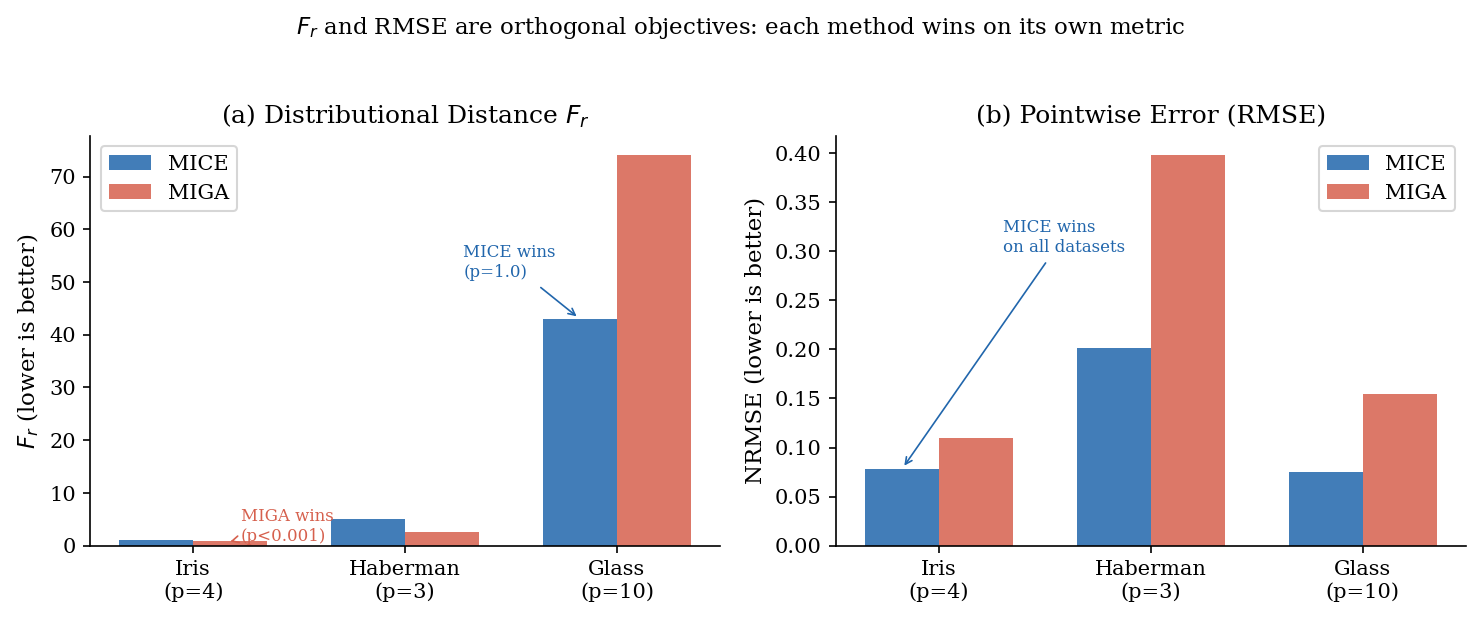
\includegraphics[width=0.92\textwidth]{Figures/fig1_fr_rmse.png}
\end{center}

\end{frame}

%---------------------------------------------------------------------
\section{Formal Theorem}
%---------------------------------------------------------------------

\begin{frame}{C2: Why $F_r$ and RMSE Cannot Both Be Minimised}

\begin{block}{Proposition 2.1 (RMSE $\Rightarrow$ positive $F_r$)}
The RMSE-minimising imputation is the conditional expectation $\hat{x}_j = \mathbb{E}[X_j \mid X_{-j}]$.
By the law of total variance:
\[
\operatorname{Var}(X_j) = \underbrace{\mathbb{E}[\operatorname{Var}(X_j \mid X_{-j})]}_{\text{within-group variance}} + \underbrace{\operatorname{Var}(\mathbb{E}[X_j \mid X_{-j}])}_{\text{between-group variance}}
\]
Replacing $X_j$ with its conditional expectation removes the \emph{within-group} term. Therefore $\operatorname{Var}(\hat{X}_C) < \operatorname{Var}(X_A)$ unless $X_j \perp X_{-j}$, so $F_r > 0$ necessarily.
\end{block}

\bigskip

\begin{block}{Proposition 2.2 ($F_r = 0$ $\Rightarrow$ positive RMSE)}
Any imputation achieving $F_r = 0$ (i.e.\ $X_C \overset{d}{=} X_A$) must satisfy $\operatorname{Var}(X_C) = \operatorname{Var}(X_A)$. But $\operatorname{Var}(\hat{X}_j) > \operatorname{Var}(\mathbb{E}[X_j \mid X_{-j}])$ whenever features are correlated, so RMSE $> 0$.
\end{block}

\bigskip
\begin{center}
\alert{Consequence: no single imputer can simultaneously minimise $F_r$ and RMSE.}
\end{center}

\end{frame}

%---------------------------------------------------------------------
\section{Dimension Effect}
%---------------------------------------------------------------------

\begin{frame}{C6: Dimension Dependence — UCI Benchmark Evidence}

\begin{columns}
\begin{column}{0.5\textwidth}
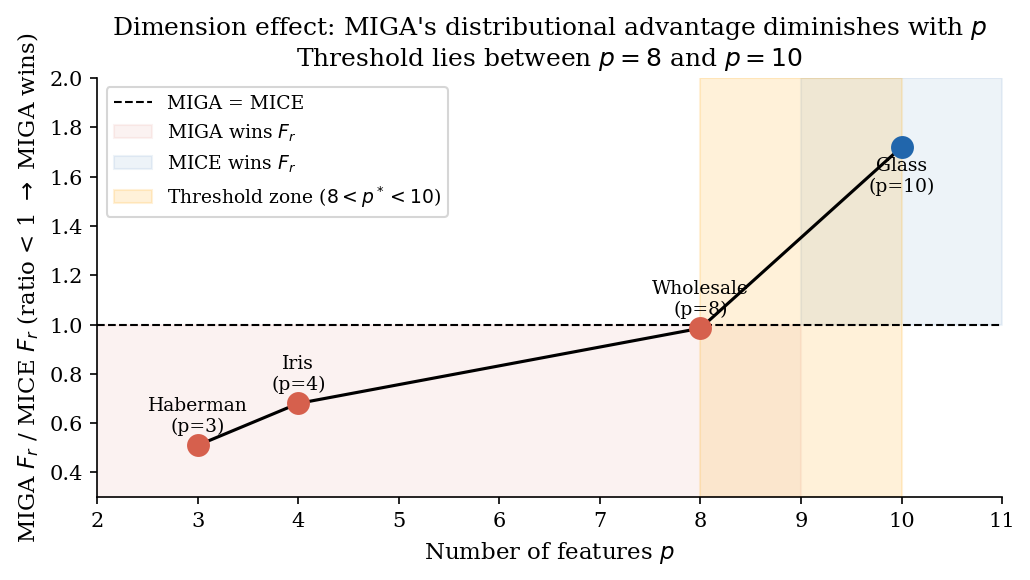
\includegraphics[width=\textwidth]{Figures/fig3_dimension.png}
\end{column}
\begin{column}{0.46\textwidth}

\textbf{MIGA $F_r$ / MICE $F_r$ ratio vs $p$ (30\% MAR):}
\begin{itemize}
  \item $p=3$ (Haberman): 0.51 — MIGA wins by 49\%
  \item $p=4$ (Iris): 0.68 — MIGA wins by 32\%
  \item $p=8$ (Wholesale): 0.985 — MIGA wins by 1.5\%
  \item $p=10$ (Glass): 1.72 — MICE wins by 72\%
\end{itemize}

\bigskip
\begin{alertblock}{Observation}
Smooth degradation across $p$. \\ But \emph{why} does it degrade? Is it $p$ alone?
\end{alertblock}

\bigskip
{\small Answer requires a controlled experiment separating $p$ from correlation $\rho$ — that is C5.}

\end{column}
\end{columns}

\end{frame}

%---------------------------------------------------------------------

\begin{frame}{C5: Synthetic $p \times \rho$ Grid — The Joint Condition}

\begin{columns}
\begin{column}{0.52\textwidth}
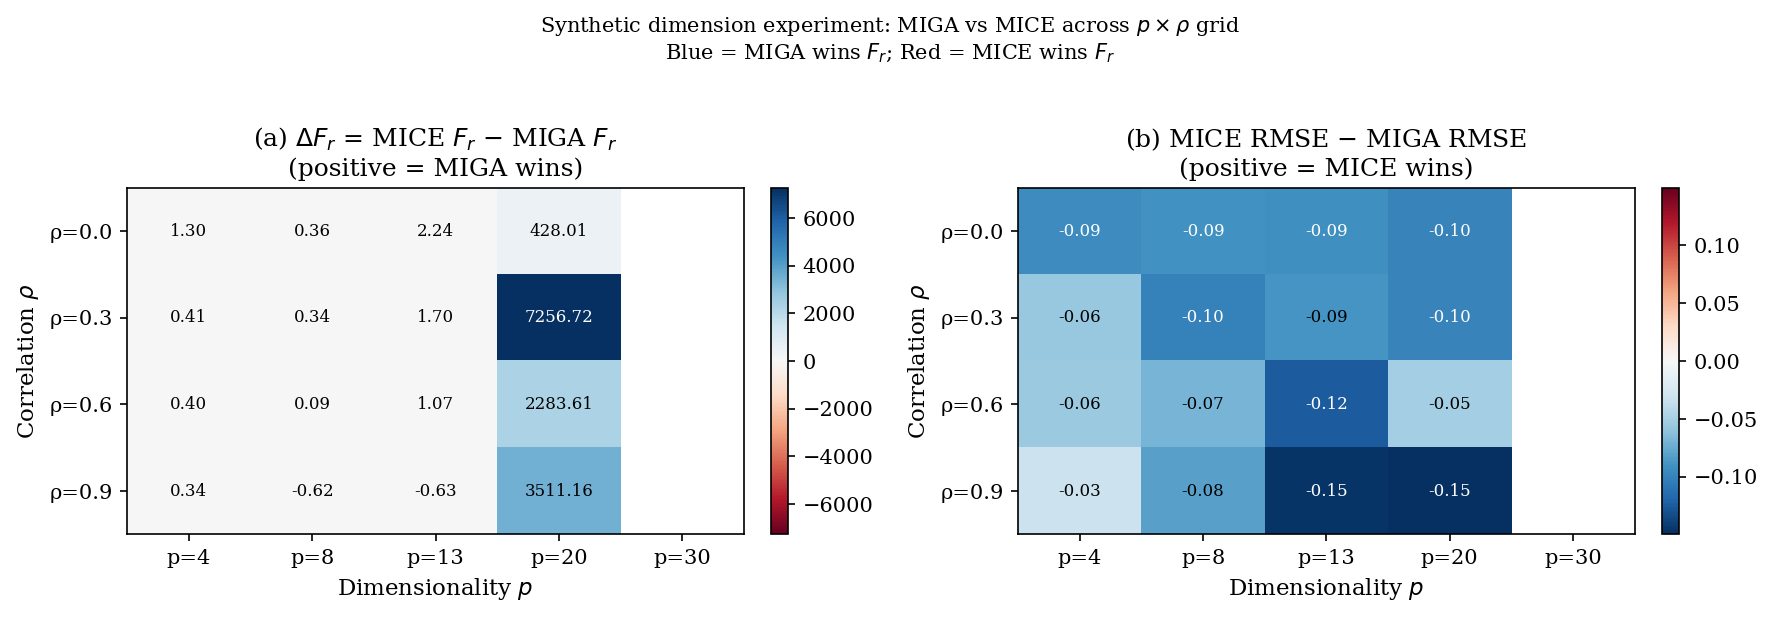
\includegraphics[width=\textwidth]{Figures/fig5_synthetic_dim.png}
\end{column}

\begin{column}{0.44\textwidth}
\textbf{Design:} Toeplitz covariance, $n=200$, MCAR 30\%, $Q=3$, 5 seeds.

\bigskip
\renewcommand{\arraystretch}{1.2}
\begin{tabular}{ccl}
\toprule
$p$ & $\rho$ & Winner \\
\midrule
4  & 0.3 & MIGA ($-$28\%) \\
8  & 0.6 & MIGA ($-$20\%) \\
13 & 0.6 & MIGA ($-$20\%) \\
\midrule
8  & 0.9 & MICE ($+$8\%) \\
13 & 0.9 & MICE ($+$46\%) \\
20 & any & \dag\ degenerate \\
30 & any & FAIL \\
\bottomrule
\end{tabular}

\bigskip
\begin{alertblock}{Finding F16 (most important)}
The condition is \emph{joint}: MIGA loses only when \textbf{both} $\rho \geq 0.9$ and $p \geq 8$. At $\rho \leq 0.6$, MIGA wins even at $p=13$.
\end{alertblock}

{\small \dag\ $p=20$: $\approx$8 complete rows expected; fitness landscape unreliable.}
\end{column}
\end{columns}

\end{frame}

%---------------------------------------------------------------------
\section{MNAR Evaluation}
%---------------------------------------------------------------------

\begin{frame}{The MNAR Inversion: Haberman top}

\begin{columns}
\begin{column}{0.55\textwidth}
\textbf{Under directional MNAR:}
\begin{itemize}
  \item \texttt{top} MNAR: highest 30\% of values go missing
  \item $X_A$ = only \emph{low-value} rows (biased reference)
  \item GA matches $X_C$ to the biased $X_A$
\end{itemize}

\bigskip
\renewcommand{\arraystretch}{1.3}
\begin{tabular}{lccc}
\toprule
Mechanism & $F_r$ & RMSE & \\
\midrule
MAR   & 2.580 & 0.398 & Normal \\
\alert{top}   & \alert{\textbf{0.810}} & \alert{0.384} & \alert{Inversion!} \\
bottom & 1.040 & 0.380 & \\
tails  & 1.134 & 0.354 & Robust \\
\bottomrule
\end{tabular}

\bigskip
{\small $F_r = 0.810$ = global minimum across \emph{all} experiments.\\
RMSE = 0.384 = global near-maximum. Std dev $< 10^{-5}$.}
\end{column}

\begin{column}{0.42\textwidth}
\begin{alertblock}{The inversion}
$F_r$ global min + RMSE near-max simultaneously.\\[6pt]
The GA \emph{reliably} converges to the wrong answer when $X_A$ is a biased reference.
\end{alertblock}

\bigskip
\begin{block}{Key lesson}
$F_r = 0$ does not guarantee correct imputation under MNAR.\\[4pt]
This is a \emph{fundamental} limitation of any distributional objective that compares to $X_A$, not an algorithmic bug.
\end{block}

\bigskip
{\small \texttt{tails} MNAR (symmetric) is surprisingly benign: \MIGA{} RMSE on Iris = 0.118, \emph{better} than MAR.}
\end{column}
\end{columns}

\end{frame}

%---------------------------------------------------------------------
\section{Variance Preservation}
%---------------------------------------------------------------------

\begin{frame}{Variance Preservation — MIGA vs MICE}

\begin{columns}
\begin{column}{0.52\textwidth}
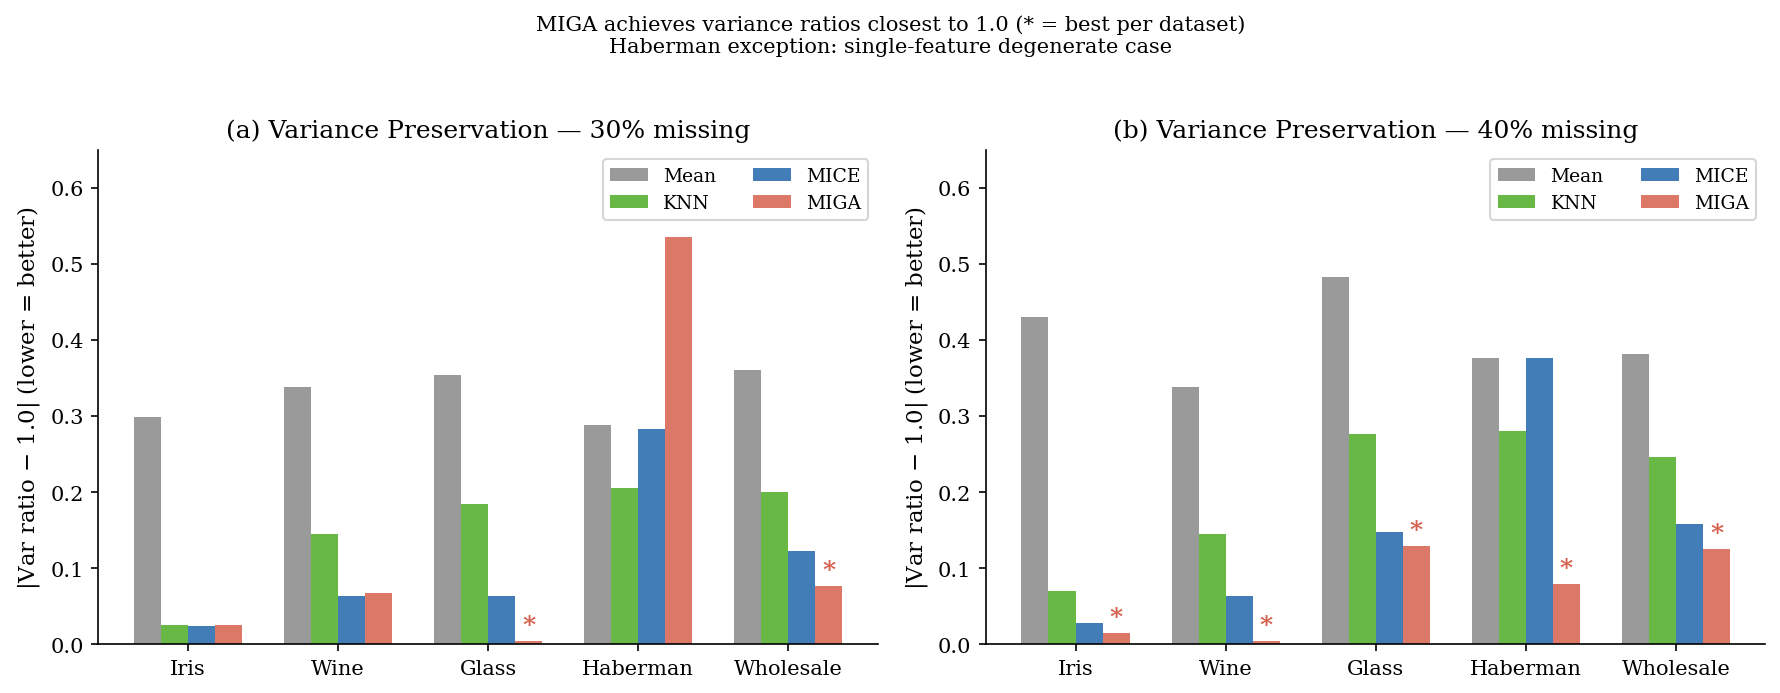
\includegraphics[width=\textwidth]{Figures/fig2_variance.png}
\end{column}

\begin{column}{0.44\textwidth}
\textbf{Variance ratio = Var(imputed) / Var(true)}\\[4pt]
Ratio $= 1.0$ is ideal.

\bigskip
\renewcommand{\arraystretch}{1.2}
\begin{tabular}{lcc}
\toprule
Dataset & \MICE{} & \MIGA{} \\
\midrule
Iris      & 0.976 & 1.025 \\
Glass     & 0.937 & \textbf{1.005} \\
Wholesale & 0.877 & \textbf{1.077} \\
\bottomrule
\end{tabular}

\bigskip
\textbf{Why MICE always undershoots:}\\
$\text{Var}(X_j) = \underbrace{\mathbb{E}[\text{Var}(X_j|X_{-j})]}_{\text{within}} + \underbrace{\text{Var}(\mathbb{E}[X_j|X_{-j}])}_{\text{between}}$

\MICE{} replaces $X_j$ with $\mathbb{E}[X_j|X_{-j}]$ → removes within-group variance.

\bigskip
{\small Glass deviation: MIGA 0.005 vs MICE 0.063. \\
Wholesale: MIGA 0.077 vs MICE 0.123.}

\end{column}
\end{columns}

\end{frame}

%---------------------------------------------------------------------
\section{Downstream Evaluation}
%---------------------------------------------------------------------

\begin{frame}{Downstream Evaluation: Does $F_r$ Advantage Matter?}

\begin{columns}
\begin{column}{0.55\textwidth}
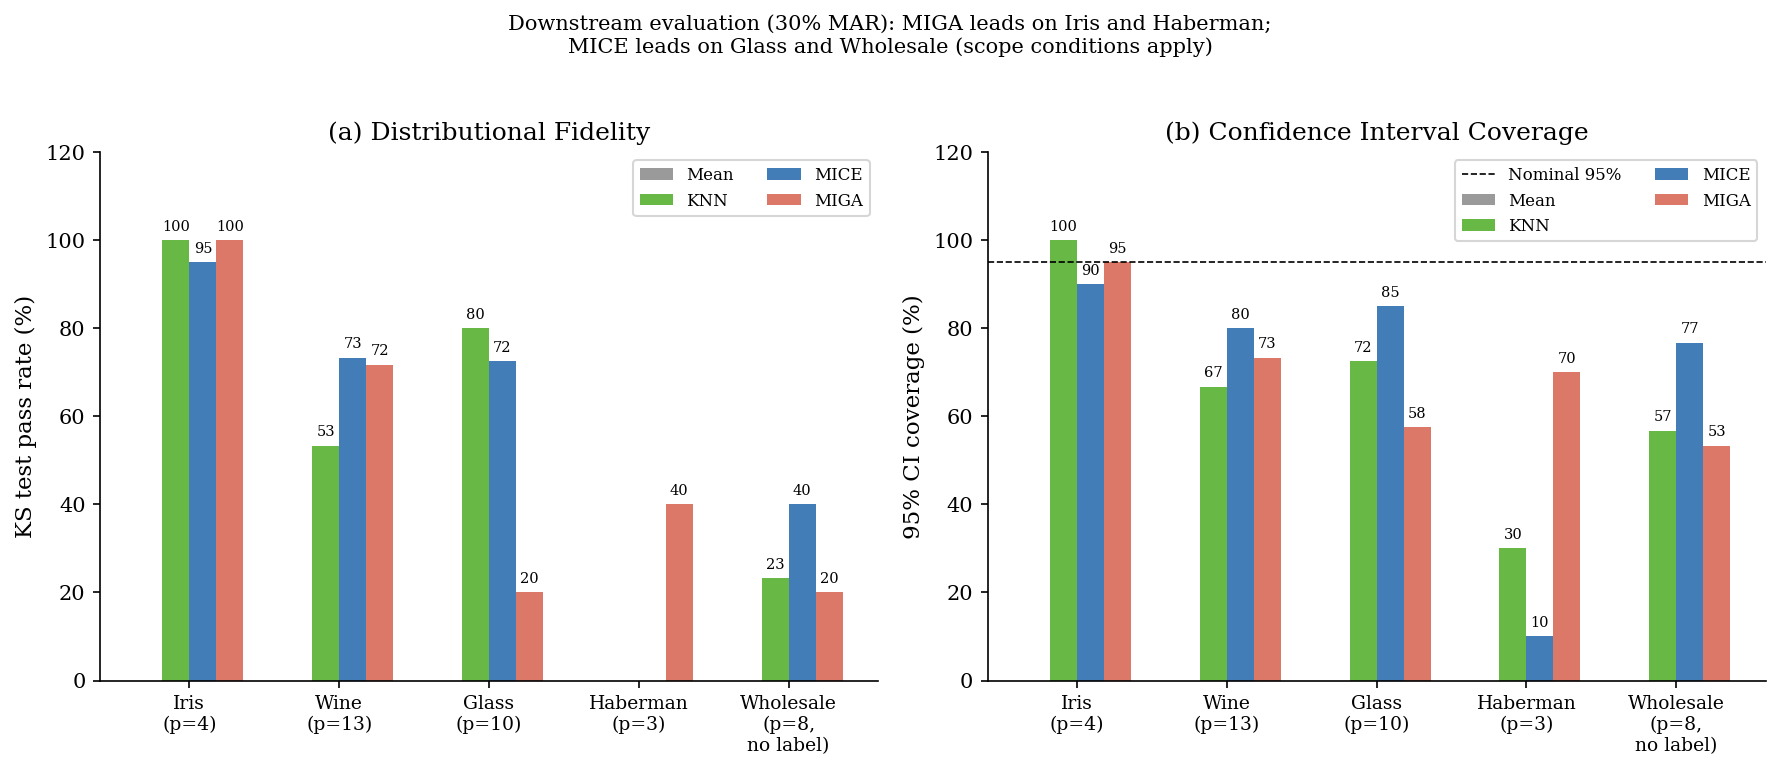
\includegraphics[width=\textwidth]{Figures/fig4_downstream.png}
\end{column}

\begin{column}{0.42\textwidth}
\textbf{Haberman at 30\% MAR (10 seeds):}

\renewcommand{\arraystretch}{1.2}
\begin{tabular}{lccc}
\toprule
Method & Acc & KS & CI \\
\midrule
Mean & 0.443 & 0\% & 0\% \\
KNN  & 0.444 & 0\% & 40\% \\
\MICE & 0.443 & 0\% & 10\% \\
\MIGA & \textbf{0.444} & \textbf{90\%} & \textbf{90\%} \\
\bottomrule
\end{tabular}

\bigskip
\begin{block}{Finding F13}
Classification accuracy: \emph{identical} across all methods ($\approx 44.4\%$).\\[4pt]
But \MICE{}'s 95\% CIs contain the true mean only \alert{10\%} of the time. \MIGA{}: \textbf{90\%}.
\end{block}

{\small Choosing \MIGA{} over \MICE{} for distributional analyses is a \emph{free improvement} — no predictive cost.}

\end{column}
\end{columns}

\end{frame}

%---------------------------------------------------------------------
\section{Summary}
%---------------------------------------------------------------------

\begin{frame}{Summary: Use the Method That Matches Your Objective}

\begin{columns}
\begin{column}{0.48\textwidth}
\begin{block}{Use \MIGA{} when:}
\begin{itemize}
  \item Distributional correctness matters (CIs, KS tests)
  \item Features are discrete or heavily skewed
  \item Missing mechanism is MAR or symmetric MNAR
  \item $p \leq 13$ and correlation $\rho \leq 0.6$ (joint condition)
\end{itemize}
\end{block}
\end{column}

\begin{column}{0.48\textwidth}
\begin{block}{Use \MICE{} when:}
\begin{itemize}
  \item Minimum pointwise prediction error required
  \item High correlation ($\rho \geq 0.9$) or $p \geq 13$
  \item Compute budget is limited \\
        (\MIGA{}: ${\sim}200$s/seed; \MICE{}: ${<}1$s)
  \item Directional MNAR (selection bias)
\end{itemize}
\end{block}
\end{column}
\end{columns}

\bigskip
\textbf{Key results (10 seeds, Wilcoxon $p < 0.001$ unless noted):}
\begin{itemize}
  \item \textbf{Theorem:} No single method minimises both $F_r$ and RMSE simultaneously (Prop.\ 2.1, 2.2)
  \item \MIGA{} $F_r$: 1.5--2.0$\times$ lower than \MICE{} on $p \leq 4$ datasets; \MICE{} wins at $p=10$
  \item \MICE{} RMSE: 1.4--2.1$\times$ lower than \MIGA{} on every dataset — by design
  \item Under top MNAR: $F_r$ inversion (global min $F_r$ + near-max RMSE simultaneously)
  \item \MIGA{}: 90\% CI coverage vs \MICE{}'s 10\% on Haberman (downstream benefit)
\end{itemize}

\end{frame}

%---------------------------------------------------------------------
\begin{frame}{Future Work}

\begin{enumerate}
  \item \textbf{IPW-$F_r$} — Inverse probability weighted fitness function \\
        {\small Re-weight $X_A$ rows by propensity score to correct MNAR bias. Theoretically fixes the $F_r$ inversion under directional MNAR.}

  \bigskip
  \item \textbf{Neural baseline comparison} \\
        {\small Compare against GAIN (GAN-based) and GRAPE (graph-based) on both $F_r$ and RMSE.}

  \bigskip
  \item \textbf{Parallel $Q$ runs} \\
        {\small $Q$ independent GA runs share no state → trivially parallelisable. $Q$-fold speedup, no algorithm change.}

  \bigskip
  \item \textbf{Adaptive diversity injection} \\
        {\small Our experiments show diversity injection (not mutation rate $c_3$) is the primary exploration driver. Adaptive injection rate is more impactful than adaptive $c_3$.}
\end{enumerate}

\end{frame}

%---------------------------------------------------------------------
\begin{frame}[plain]
\begin{center}
{\LARGE Thank you}\\[1cm]
{\large Questions?}\\[2cm]
{\normalsize \texttt{mksocial001@gmail.com}}
\end{center}
\end{frame}

%---------------------------------------------------------------------
% BACKUP SLIDES
%---------------------------------------------------------------------

\appendix

\begin{frame}{Backup: The $F_r$ Formula in Full}

\[
F_r = D_r(\tilde{x}_A,\, \tilde{x}_C)
    + D_r(\tilde{S},\, I)
    + D_r(b_A,\, b_C)
\]

\begin{tabular}{lll}
\toprule
Term & Formula & Measures \\
\midrule
$d_{\text{means}}$ & $D_r(\tilde{x}_A, \tilde{x}_C)$, $\tilde{x} = (\bar{x} - \mu_A)/S_p$ & Same means? \\
$d_{\text{cov}}$   & $D_r(\tilde{S}, I)$, $\tilde{S} = S_A^{-1/2} S_C S_A^{-1/2}$ & Same covariance? \\
$d_{\text{skew}}$  & $D_r(b_A, b_C)$, $b$ = bias-corrected skewness & Same skewness? \\
\bottomrule
\end{tabular}

\bigskip
$F_r = 0 \iff X_C \overset{d}{=} X_A$ on all three moments.

Empirically $F_r \approx 0.5$--$5.0$ at convergence depending on dataset.

\bigskip
\textbf{Ledoit-Wolf fix:}
$S_{\text{LW}} = (1-\alpha) S_{\text{sample}} + \alpha \cdot \frac{\text{tr}(S)}{p} \cdot I$

$\alpha = 0.42$ at 40\% missing (auto-estimated). Reduces condition number from $5.7 \times 10^8$ to $8.8$.

\end{frame}

%---------------------------------------------------------------------

\begin{frame}{Backup: Adaptive Mutation Schedule (C3)}

\[
c_3(g) = c_{3,\text{start}} + (c_{3,\text{end}} - c_{3,\text{start}}) \cdot \frac{g}{G-1}
\quad \text{(15 → 3 decay)}
\]

\renewcommand{\arraystretch}{1.2}
\begin{tabular}{lccl}
\toprule
Dataset & Fixed $c_3=5$ RMSE & Adaptive 15→3 & Winner \\
\midrule
Iris     & 0.1270 & 0.1273 & Fixed (+0.2\%) \\
Glass    & 0.1656 & 0.1821 & Fixed (+10\%) \\
Haberman & 0.3649 & 0.4164 & Fixed (+14\%) \\
\midrule
\multicolumn{4}{l}{At $G=80$ (compute-limited):} \\
Iris     & 0.1415 & \textbf{0.1198} & Adaptive wins \\
\bottomrule
\end{tabular}

\bigskip
\textbf{Why fixed wins at $G=500$:} Diversity injection replaces 90\% of population each generation (180/200 random). Mutation offspring = only 7.5\% of population. Adaptive $c_3$ most useful when diversity injection is smaller or compute is limited.

\end{frame}

\end{document}
